\chapter*{Prefácio}
\addcontentsline{toc}{chapter}{Prefácio}


O \sage é um poderoso software para a manipulação de objetos matemáticos.
É um software gratuito e de código aberto, sob a licensa GPL, construído
sobre diversos outros pacotes, também de código aberto, como o NumPy, 
SciPy, matplotlib, Maxima, GAP, R, etc.  Baseado na linguagem de programação
Python é uma ótima ferramenta para explorar conceitos matemáticos. 

Nesse texto usamos o \sage para explorar a área da matemática
conhecida como teoria dos números, ou aritmética. O \sage possui
uma enorme gama de recursos relacionados à teoria dos números
básica, além de dispor de métodos que auxiliam a construção de
ferramentas para nossas próprias investigações.

Sendo baseado em Python, o \sage consegue executar qualquer
comando ou script Python da forma esperada (a menos
de um conjunto de medida nula). 
Com o risco de exagerarmos no tom informal, tentamos evitar ao máximo
o uso conhecimentos prévios sobre a linguagem Python e sobre
algoritmos de uma forma geral. Evidentemente, alguns
conceitos e técnicas apresentados fazem uso de conhecimentos 
específicos de algoritmos, mas \textbf{não é necessário
saber programar} para seguir essas notas, basta estar disposto
a aprender.

Aproveitamos para destacar que existe uma 
enorme quantidade de recursos do \sage que não
abordaremos em detalhes, como o cálculo simbólico, a construção de gráficos 
integrado ao matplotlib, objetos da álgebra abstrata,
como grupos e aneis, combinatória, computação numérica...
Dessa forma, instigamos ao leitor que faça um passeio
pela documentação do \sage (\cite{sagedoc}) e descubra outras ferramentas
disponíveis que podem auxiliá-lo no seu dia a dia de estudante
ou professor, além da documentação dos recursos, também há diversos
tutoriais ou materiais sobre temas específicos e uma lista é mantida
com os livros e publicações sobre o \sage.
Recomendamos também o ótimo livro \cite{sagesbm},
única referência em português sobre o \sage de conhecimento
do autor. Em inglês há mais recursos, destacamos
\cite{zimmermann2018computational} (Versão em inglês, original
francês) e \cite{bard2015sage} (Versão em inglês, também
disponível em espanhol), ambos com versões gratuitas 
disponíveis nos sites dos autores e contendo ao menos
um capítulo sobre teoria dos números..



SEPARADOR

Ao escrever essas notas fizemos algumas escolhas sobre o estilo e o conteúdo
que necessitam justificativa.
Com o intuito de não tornar esse texto mais longo que deveria, optamos
por omitir algumas demonstrações e discussões
mais teóricas, indicando referências mais adequadas
(e decerto mais bem escritas) para o que for omitido. Dessa forma, essas notas 
não tem como objetivo substituir um texto mais formal de teoria dos números,
com todas as propriedades, teoremas e demonstrações.
A exceção  ocorre quando as demonstrações são, de alguma forma, construtivas.
Nesse caso procuramos fornecer um esboço da demonstração que
auxilie na construção de um código \sage.

Apesar do nosso objetivo principal ser a apresentação do \sage
como uma ferramenta pronta para o uso, também gostaríamos que
o leitor desenvolvesse um raciocínio lógico que o permita
transpor uma lista simples de procedimentos em linguagem matemática
para código \sage. Para tal iremos apresentar a construção de algumas
ferramentas básicas que já estão implementadas no sage, então, sim,
em alguns momentos estaremos \emph{reinventando a roda}, mas cremos
que esse é um passo importante para o entendimento dos 
algoritmos mais avançados que apresentaremos ao final do texto.

Para os que já são familiarizados com a linguagem Python, inserimos algumas
observações onde o \sage supostamente funciona de forma diferente do Python,
ou onde objetos ligeiramente diferentes são usados.
Para os que não são familiarizados com o \sage ou Python, optamos por
não inserir uma longa seção  inicial tratando de sintaxe,
lógica de programação, etc. Vamos direto ao ponto e espalhamos essas explicações
aqui e ali, na medida que se fazem necessárias. Para os leitores
mais sistemáticos, os três primeiros
capítulos do já citado \cite{sagesbm} fornecem uma introdução
completa ao \sage, sugerimos sua leitura antes de explorar
esse texto.

{\color{blue} Descrição capítulo a capítulo}

Inserimos em cada capítulo uma seção 
chamada \textbf{Explore!}, onde descrevemos
alguns tópicos adicionais
que acreditamos serem aplicações interessantes. Dentro
de cada tópico há alguns
exercícios mas, para alguns deles,  o instrutor pode desenvolver miniprojetos
estendendo o escopo abordado. No final de cada capítulo
há uma seção \textbf{Exercícios}, com problemas adicionais,
generalizações de resultados ou implementações alternativas
às mostradas no corpo do texto. Tais exercícios
não são, em geral, fundamentais para a
compreensão do assunto. Por outro lado, no corpo do texto
há determinados exercícios que julgamos essenciais
para o desenvolvimento da aprendizagem, alguns,
inclusive, podem não fazer muito sentido se ignorados e
deixados para depois.
Tentamos indicar
os exercícios mais trabalhosos ou que exigem um 
aprofundamento das técnicas com um sinal X, no entanto
nenhum requer assuntos não abordados, exceto 
menção explícita a alguma referência.


\mainmatter

\chapter*{Introdução}
\addcontentsline{toc}{chapter}{Introdução}

\section*{O \sage}

Apresentamos brevemente como utilizar o \sage e alguns conceitos
básicos.

Há diversas formas de se trabalhar com o \sage, e uma de suas vantagens
é que você nem precisa ter o \sage instalado em seu computador 
para usá-lo. Na prática, não há muitas razões para a maior parte
dos usuários instalar o \sage. 

De toda forma, se optar pela
instalação, siga as instruções em \url{https://www.sagemath.org/download.html}.
Após a instalação a forma mais direta de utilização é através
da linha de comando: abra uma linha de comando, digite \ils{sage}
e, voilá, você já está dentro do interpretador interativo \sage.
Tente digitar algum código

\begin{sageinput}
2+2
\end{sageinput}
\begin{sageoutput}
4
\end{sageoutput}

Usaremos o padrão acima nessas notas, o texto no quadro azul
é o código \sage e o texto no quadro verde é o resultado do código
acima. 
No interpretador \sage, qualquer código sage válido inserido
será executado e você verá o resultado na hora. Para 
códigos mais elaborados o mais usual é salvá-lo em um arquivo com a extensão
\ils{.sage} e executar o comando \ils{sage} na linha de comando
com o arquivo como argumento. No entanto, a interface mais amigável para o
\sage é fornecida pelo Jupyter, um projeto para o desenvolvimento de padrões
para computação interativa. Ao utilizar o \sage em um notebook Jupyter
você vai trabalhar em um página web local, através do seu navegador,
como na Figura \ref{fig:jupyter}.

\begin{figure}[h]
  \centering
  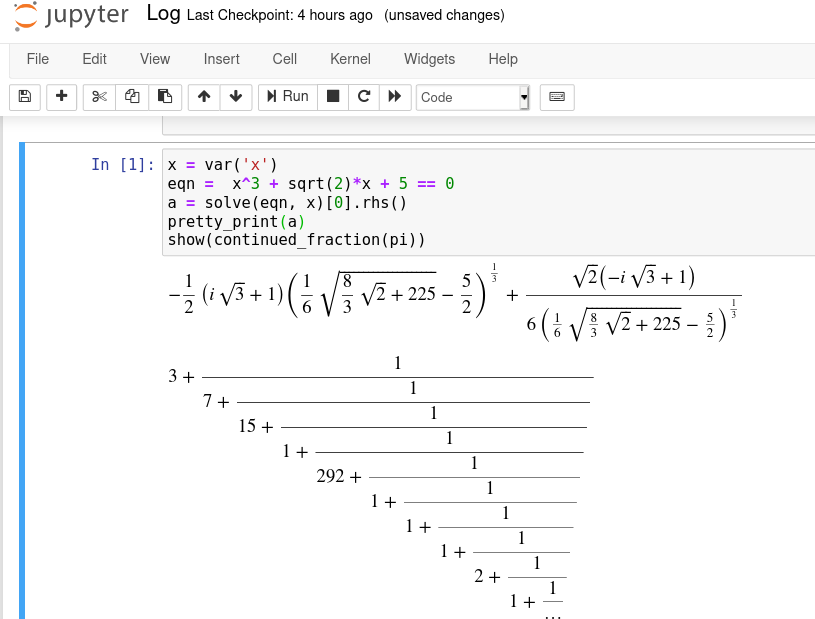
\includegraphics[scale=0.4]{imgs/jupyter.png}
  \caption{Tela do \emph{Jupyter}}
  \label{fig:jupyter}
\end{figure}

Par a maior parte das pessoas, no entanto, recomendamos
a utilização de alguma opção \emph{online} do \sage. Há duas
opções principais. A mais simples e direta de todas é utilizar
a célula de cálculo no site \emph{SageMathCell}, 
acessado em \url{https://sagecell.sagemath.org}. Nesse site
você verá um campo de texto onde pode inserir código \sage. Em
seguida basta clicar em \emph{Evaluate} para ver o resultado,
como na Figura \ref{fig:sagemathcell}.  Todos os códigos
utilizados nesse texto podem ser executados no
\emph{SageMathCell}. Vale destacar, no entanto, que ao fechar o site
todo o seu código será perdido, bem como o resultado. Dessa forma
se quiser salvar o seu trabalho, você pode copiar o código que digitou
no \emph{SageMathCell} e salvar em um arquivo de texto, podendo
voltar a trabalhar nele em outro momento.

\begin{figure}[ht]
  \centering
  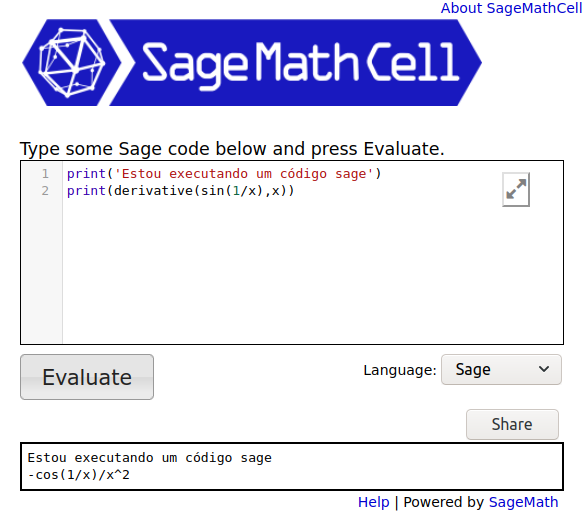
\includegraphics[scale=0.4]{imgs/sagemathcell.png}
  \caption{Tela do SageMathCell}
  \label{fig:sagemathcell}
\end{figure}

Outra opção, que evita o problema de perder os códigos, é usar
o \emph{CoCalc}, uma plataforma online permitindo o uso
de diversas ferramentas, incluindo o \sage. Apesar de existirem 
diversos planos pagos, fornecendo mais capacidade
de memória e processamento, há uma
versão gratuita que é o suficiente para grande parte
das aplicações. Ao criar uma conta no site do \emph{CoCalc}, 
você poderá criar arquivos e projetos de diversos tipos. 
Estaremos interessado em particular em \emph{worksheets \sage},
arquivos no formato \ils{.sagews}, que funcionam de forma parecida
com notebooks do Jupyter\footnote{também é possível usar o Jupyter
com o \sage dentro do Cocalc}. A grande vantagem é que os
seus arquivos ficarão salvos na sua conta, mesmo após o
fechamento do navegador, além disso você pode trabalhar
colaborativamente com outros colegas no mesmo arquivo.

\begin{figure}[h]
  \centering
  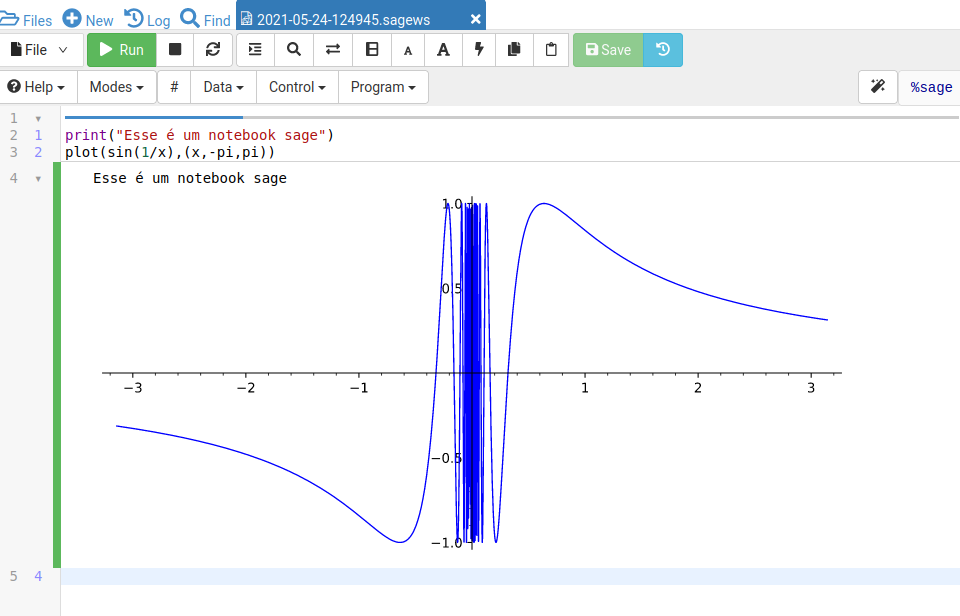
\includegraphics[scale=0.4]{imgs/cocalc.png}
  \caption{Tela do \emph{CoCalc}}
  \label{img:cocalc}
\end{figure}


O \emph{CoCalc} e o \emph{Jupyter} fornecem diversas outras
ferramentas, recomendamos que o leitor acesse os sites
dessas plataformas e descubra quais dessas ferramentas pode
achar útil. Como comentamos, para essas notas, o uso
do \emph{SageMathCell} será suficiente.


Vemos a seguir alguns conceitos básicos sobre o \sage. 


\paragraph{Conjuntos Numéricos} Os objetos mais básicos
que utilizaremos serão os números. Sabemos que o número
$12$, por exemplo, é um número inteiro, racional, real
e complexo. No \sage, no entanto, faz certa
diferença onde os números estão sendo considerados. Não
fará sentido, por exemplo, perguntar ao \sage 
a fatoração em primos de \ils{12.0}, pois o número $12$,
inserido dessa forma, com o \ils{.0}, será considerado como um número real.
No entanto, pedir a fatoração em primos de \ils{12} 
retorna o resultado esperado. Os recursos disponíveis e as operações
irão portanto depender do \emph{tipo} do objeto considerado.
Vejamos como definir alguns tipos números e verificamos o tipo
dos objetos gerados usando a função \ils{parent}. No \sage, 
a unidade imaginária $i = \sqrt{-1}$ pode ser
inserida usando a letra \ils{I}.
\begin{center}
\begin{tabular}{rl}
  Código & Resultado \\ \hline
  \ils{parent(5)} & Integer Ring\\
  \ils{parent(5/3)} & Rational Field \\
  \ils{parent(5.12)} & Real Field with 53 bits of precision \\
  \ils{parent(5+3*I)} & Symbolic Ring
\end{tabular}
\end{center}

O último resultado não foi bem o esperado, ele ficará
mais claro no Parágrafo \textbf{Sequências Recorrentes
e Expressões Simbólicas} na Seção \ref{par:fib} (mas, se ainda
estiver desconfiado, calcule \ils{I\^{}2}). Podemos 
tentar converter um número de um tipo para outro usando
a \emph{coerção}\index{Coerção}. Para isso usaremos \ils{ZZ} para os inteiros, \ils{QQ} para
os racionais, \ils{RR} para os reais e \ils{CC} para os complexos. 
Vamos tentar converter alguns números de um conjunto para o outro
. Assumiremos que você executará o código abaixo, e todos os demais nessas notas,
em uma célula como no \emph{SageMathCell}. Nesse tipo de célula você
pode escrever várias linhas de código ao mesmo tempo. O \sage
irá executar todas, no entanto só exibirá o resultado
da última linha. Para forçar a exibição usamos a função \ils{print}.
\begin{sageinput}
print(QQ(5.12))
print(parent(QQ(5.12)))
print(RR(1/7))
print(QQ(pi))
\end{sageinput}
\begin{sageoutput}
128/25
Rational Field
0.142857142857143
------------------------------------------------------------
TypeError                  Traceback (most recent call last)
# ...  GRANDE MENSAGEM DE ERRO... #
TypeError: unable to convert pi to a rational
\end{sageoutput}

Uma função muito parecida com a função \ils{print}
é a função \ils{show}\index[sage]{\ils{show}}, ela exibe o resultado
de forma mais bonita, principalmente objetos matemáticos:
enquanto \ils{print(QQ(5.12))} exibe \ilso{128/25},
\ils{show(QQ(5.12))} exibe $\frac{128}{25}$.

Destacamos que a aritmética nos inteiros e nos racionais
acontece de forma exata\footnote{Para os conhecedores
de Python: no \sage, o operador \ils{/} entre inteiros 
retorna um objeto  do tipo \ils{Rational}, um número
racional. Para obter o resultado como ponto flutuante
ou número real do \sage use  \ils{float(a/b)} ou 
\ils{RR(a/b)}, respectivamente.}.
 Por outro lado, como números
reais, e complexos, em geral tem representação decimal 
infinita, não é possível armazená-los completamente na
memória do seu computador. Dessa forma, o \sage (e qualquer
outro sistema) usa uma aproximação do número
real com uma precisão pré-determinada, chamada
de \emph{ponto flutuante}\index{Ponto flutuante}.
É possível aumentar
arbitrariamente a precisão considerada.
\begin{sageinput}
print(RR(e))
RR100 = RealField(prec=100)
print(RR100)
print(RR100(e))
\end{sageinput}
\begin{sageoutput}
2.71828182845905
Real Field with 100 bits of precision
2.7182818284590452353602874714
\end{sageoutput}
É preciso um pouco de cautela ao trabalhar com números reais.
Considere os números $1+10^{-20} \neq 1+2\times 10^{-20}$. 
Veja o que ocorre quando o comparamos como elementos
do \ils{RR} com a precisão padrão do \sage e com o 
\ils{RR100} que definimos acima\footnote{O
\ils{prec=100} não significa que tais números
reais terão precisão de $100$ dígitos decimais, e sim
$100$ bits.}.

\begin{sageinput}
RR(1+10^(-20)) == RR(1+2*10^(-20))
RR100(1+10^(-20)) == RR100(1+2*10^(-20))                      
\end{sageinput}
\begin{sageoutput}
True
False
\end{sageoutput}

\paragraph{Operações básicas}

Como é de se esperar, podemos fazer as operações
básicas com os números, e, em alguns casos, até com outros objetos. Usamos
o \ils{*} para o produto, o \ils{/} para divisão ---
embora isso possa não retornar o resultado esperado ---
e, ao contrário do Python, usamos \ils{\^{}} para exponenciação.
A ordem das operações segue a convenção usual, no entanto
recomendamos o uso de parenteses mesmo quando não for necessário.
Assim $1 + \frac{2\times 3+1}{1+\frac{1}{2^3}}$, por
exemplo, se escreveria como
\ils{1+(2*3+1)/(1+(1/(2\^{}3)))}



\paragraph{Listas}


Um dos tipos de objetos mais importantes que usaremos
no \Sage é a lista. Uma lista pode ser pensada como
uma sequência finita de elementos que podem
ser acessados pela posição, chamada de \emph{índice}, sendo
o primeiro elemento o elemento de índice $0$, o 
segundo de índice $1$, etc. No \Sage usamos colchetes
para definir listas e para recuperar seus elementos. Os comandos 
a seguir mostram algumas propriedades da lista. 

\begin{sageinput}
L = ["Euler", "Gauss", "Germain"]
"Gauss" in L
\end{sageinput}
\begin{sageoutput}
True
\end{sageoutput}

\begin{sageinput}
L[0]; L[2]
\end{sageinput}
\begin{sageoutput}
'Euler'
'Germain'
\end{sageoutput}

É importante destacar que listas no \Sage \textbf{não são conjuntos},
já que eles podem ter elementos repetidos e a ordem dos elementos importa.
No entanto, na prática usaremos listas como conjuntos nas nossas
aplicações, principalmente pela facilidade de se recuperar elementos
\footnote{Existe uma forma de se trabalhar com conjuntos
no \Sage mas, por enquanto, isso não nos será muito útil}.

Uma das técnicas mais úteis para se definir uma lista em \Sage é através
da compreensão de lista. A compreensão de listas é muito natural
para nós matemáticos pois tem a estrutura parecida com a
definição de um conjunto a partir de outro. Por exemplo, poderíamos
definir o conjunto dos $5$ primeiros quadrados perfeitos como
$\{n^2 \mid n \in\{ 1, 2, 3, 4, 5\}\}$. No \Sage isso pode ser feito assim:

\begin{sageinput}
[n^2 for n in [1..5]]
\end{sageinput}
\begin{sageoutput}
[1, 4, 9, 16, 25]
\end{sageoutput}

Se quiséssemos agora calcular o fatorial dos 
$5$ primeiros quadrados perfeitos, bastaria usar a lista já criada:
\begin{sageinput}
Q = [n^2 for n in [1..5]]
[factorial(x) for x in Q]
\end{sageinput}
\begin{sageoutput}
[1, 24, 362880, 20922789888000, 15511210043330985984000000]
\end{sageoutput}

A notação \ils{[a..b]} cria uma lista que funciona
como o conjunto $\{a,a+1,\dots,b\}$. Uma outra forma
de criar listas de números é utilizar a função
 \ils{srange(x)}, que cria uma lista que funciona como o
conjunto $\{0,\dots,x-1\}$ quando $x\geq 0$ é inteiro.
Podemos também adicionar um parâmetro a mais para começar de 
outro inteiro diferente do zero. Veja:
\begin{sageinput}
srange(-5,5)
\end{sageinput}
\begin{sageoutput}
[-5, -4, -3, -2, -1, 0, 1, 2, 3, 4]
\end{sageoutput}
Note que, em ambos os casos, a lista gerada pelo
\ils{srange} não inclui o último elemento, de forma
que \ils{[a..b]} e \ils{srange(a,b+1)} geram
a mesma lista, assim como \ils{[0..x]} e
\ils{srange(x+1)}. A função \ils{srange} também
permite alguns parâmetros adicionais que nos
serão úteis mais adiante
\footnote{Para os conhecedores de Python:
existem algumas diferenças entre o \ils{srange}
e o \ils{range} usual. A mais importante é que
os números de uma lista gerada com \ils{srange}
são inteiros da classe \ils{Integer}, e não
da classe \ils{int} do Python. Isso significa
que os métodos específicos da classe \ils{Integer}
não irão funcionar em inteiros gerados usando 
o \ils{range} usual.}.

Listamos alguns métodos e funções de listas que
usaremos com frequência. Usamos a lista
\ils{L = [1,2,3]} nos exemplos, os métodos
não retornam uma lista nova, e sim alteram a 
lista \ils{L} (efeitos não acumulativos, i.e. redefinimos a lista \ils{L} 
em cada linha)
{\renewcommand{\arraystretch}{1.3}
\begin{table}[h]
\centering
  \begin{tabular}{llll}
     & Definição &  Exemplo & Resultado \\ \hline
    \ils{min} & Menor elemento & \ils{min(L)} & 
            \ilso{1} \\ \hline
    \ils{max} & Maior elemento & \ils{max(L)} & \ilso{3} \\ \hline
    \ils{sum} & Soma & \ils{sum([1..6])} & \ilso{21} \\ \hline
    \ils{prod} & Produto & \ils{prod([1..5])} & \ilso{120} \\ \hline
    \ils{sorted} & Ordena & \ils{sorted([1,-1,2,-12])} & \ilso{[-12, -1, 1, 2]} \\ \hline
    \ils{.append} & Insere no final & \ils{L.append(5)} &
            \ils{L} $\to$ \ilso{[1,2,3,5]} \\ \hline
    \ils{.remove} & Remove 1ª ocorrência & \ils{L.remove(2)} &
            \ils{L} $\to$ \ilso{[1,3]} \\
     & \ils{Lr = [1,2,3,2,4]} & \ils{Lr.remove(2)} & 
            \ils{Lr} $\to$ \ilso{[1,3,2,4]} \\ \hline
    \ils{.pop} & Remove por índice & \ils{L.pop(0)} & 
            \ils{L} $\to$ \ilso{[2,3]} \\ \hline
    \ils{.reverse} & Inverte ordem &  \ils{L.reverse()} & 
            \ils{L} $\to$ \ilso{[3,2,1]}
  \end{tabular}
\end{table}}


\paragraph{If (else, elif), for, while}

Apresentamos, brevemente, alguns conceitos que utilizaremos
sobre a estrutura dos nossos códigos. Ao se deparar com 
um código, o \sage irá executar os comandos sequencialmente, da
primeira até a última linha.  Há duas formas principais de alterarmos
essa ordem, utilizando condicionais ou laços de repetição. Um
\emph{condicional} \index{Condicional (If)} permitirá que você possa
determinar comportamentos diferentes
dependendo se uma condição for válida ou não. Em (quase?) toda
linguagem de programação o condicional usa a palavra em inglês 
\ils{if}, que significa \emph{se}. A sintaxe é a seguinte:
\begin{sageinput}
if (condicao):
  Comando #1
  Comando #2
  Comando #3
Comando #4
\end{sageinput}
Note que alguns comandos estão com um espaçamento diferente. O nome
disso é \emph{indentação}\index{Indentação}, esses comandos estão mais afastados do início
da linha, e no mesmo nível, justamente para indicar ao \sage o que deve ser executado caso
a condição seja verdadeira. No exemplo acima, seriam executados
os comandos \#1, \#2 e \#3 caso a condição seja verdadeira. O comando \#4
não está com a mesma indentação dos anteriores, dizemos que ele está \emph{fora
do }\ils{if}, portanto ele será executado sempre, mesmo que a condição seja falsa.
A \ils{condicao} é um pedaço de código que o \sage consiga
testar se é verdadeiro ou falso. Formalmente, existe um tipo de objeto,
chamado \emph{booleano}, que assume dois valores diferentes, \ils{True}
para verdadeiro e \ils{False} para falso. Ao se deparar com um
comando \ils{if} como acima, o \sage tenta transformar a condição
em um valor booleano. Na tabela abaixo mostramos os testes mais
comuns usados em condições. 
\begin{center}{\renewcommand{\arraystretch}{1.2}
\begin{tabular}{llll}
  \sage & Condição & Exemplo & Resultado\\ \hline
  \ils{a == b} & $a$ igual à $b$ & \ils{1 == 3} & \ilso{False} \\
  \ils{a > b} & $a$ maior que $b$ & \ils{2 > pi} & \ilso{False} \\
  \ils{a >= b} & $a$ maior ou igual à $b$ & \ils{2 >= 2} & \ilso{True} \\
  \ils{a < b} & $a$ menor que $b$ & \ils{2 < 2} & \ilso{False} \\
  \ils{a <= b} & $a$ menor ou igual à $b$ & \ils{2 <= 7} & \ilso{True} \\  
  \ils{a=!b} & $a$ diferente de $b$ & \ils{1!=2} & \ilso{True} \\
  \ils{a in L} & $a$ está na lista $L$ & \ils{3 in [2,4,6]} & \ilso{False} \\
  \ils{not P} & negação de $P$, não $P$ & \ils{not (1 == 2)} & \ilso{True}
\end{tabular}}
\end{center}
Você pode testar alguns desses valores
substituindo o valor  de \ils{a} e \ils{b} ou de algumas constantes.
Mas antes leia as seguintes observações:
\begin{itemize}
  \item Note que utilizamos \ils{==} para comparar dois objetos. De fato, o \ils{==}
  tem um significado diferente do sinal de igual simples \ils{=} que utilizamos
  anteriormente. O sinal de igual funciona como atribuição: Ao escrever \ils{a = 2}
  estamos atribuindo ao \ils{a} o valor $2$ (matematicamente, seria como
  escrever \textit{`Seja $a = 2$'} ou \textit{`Tome $a = 2$'})  . Enquanto que o \ils{==} serve
  apenas para testar se dois objetos são iguais,
  de forma que \ils{a == 2} é um objeto do tipo \ils{bool} que tem apenas
  dois valores: \ils{True} se \ils{a} for $2$ ou \ils{False} caso contrário
  \footnote{Se \ils{x} já existe,
  \ils{x=x+1} faz sentido pois estamos atribuindo à \ils{x} o valor do seu sucessor
  (teste!), enquanto que \ils{x == x+1} é um teste que deveria
  retornar sempre \ils{Falso} já que nenhum \emph{número} é igual ao seu sucessor... 
  ou é? (Dica: no \sage existe o \ils{Infinity}. Quanto é $\infty + 1?$)}.
  \item O comportamento de algum desses operadores pode parecer estranho
  quando envolvem expressões simbólicas (descobriremos mais adiante o que
  isso significa) ou outros objetos. No entanto, com números você
  não deve ter problemas e obter o resultado esperado.
  \item Na última linha da tabela utilizamos o \ils{not} para negar
  logicamente o valor de uma outra condição \ils{P}. Também é possível
  fazer outras operações entre condições usando o \ils{and} (e) e
  \ils{or} (ou).
\end{itemize}

Também é possível passar ao \sage um outro bloco
de comandos a ser executado caso a condição seja
falsa, com o \ils{else}, ou testar várias condições simultaneamente
com o \ils{elif}. Nos reservamos a comentar esses comandos
na medida que forem necessários.

% Por exemplo, pode
% ser interessante saber se um número é não negativo antes de calcular
% sua raíz quadrada. Assim, testamos primeiramente se o número é $\geq 0$,
% e caso ver

% \begin{sageinput}
% n = 10
% if (n >= 0):
%   print(RR(sqrt(n)))
% \end{sageinput}
% \begin{sageoutput}
% 3.16227766016838
% \end{sageoutput}

Outra forma de mudar a ordem usual de uma lista de comandos é
utilizar um laço de repetição. O primeiro laço de repetição
que apresentaremos é o \ils{for}, usado quando
gostaríamos de repetir um bloco de comandos enquanto uma variável
varia em uma lista de elementos. A sintaxe é dada por
\begin{sageinput}
for obj in L:
  Comando #1
  Comando #2
  ...
\end{sageinput}
\noindent Onde \ils{L} é uma lista (ou outro objeto iterável). Nesse exemplo,
inicialmente \ils{obj} assume o valor do primeiro elemento da lista,
em seguida os comandos do bloco são executados, ao chegar no final
do nível de indentação, atribui-se ao \ils{obj} o segundo elemento da lista
e voltamos ao Comando \#1, isso ocorre tantas vezes quanto há elementos
na lista \ils{L}, em cada repetição, chamada de \emph{iteração}, o valor
de \ils{obj} é um valor diferente da lista. Quando a lista acaba o 
programa \emph{sai do }\ils{for} e os comandos da indentação
anterior continuam a ser  executados. 
\begin{sageinput}
matematicos = ["Euler","Gauss","Dirichlet"]
for m in matematicos:
  print("{} foi um matematico".format(m))
\end{sageinput}
\begin{sageoutput}
Euler foi um matematico
Gauss foi um matematico
Dirichlet foi um matematico
\end{sageoutput}

O \ils{for} é particularmente
útil quando queremos que um bloco de comandos se repita uma quantidade
predeterminada de vezes. Por exemplo, se quisermos exibir uma mesma mensagem
3 vezes, usamos
\begin{sageinput}
for i in [1..3]:
  print("OI")
\end{sageinput}
\begin{sageoutput}
OI
OI
OI
\end{sageoutput}

O outro laço de repetição que nos será particularmente útil é chamado
de \ils{while}. O \emph{while}, enquanto em português, funciona
como o \ils{if}: fornecemos uma condição a ser testada e, caso 
a condição seja verdadeira, um bloco de comandos será
executado. No entanto, ao final do bloco de comandos, 
a condição será testada novamente, em seguida, se ainda for
verdadeira, o bloco será novamente executado. Esse processo
se repetirá enquanto a condição for verdadeira. Quando a 
condição for falsa, o bloco não é executado e programa
segue a execução normal das linhas posteriores. 
A sintaxe é a seguinte:
\begin{sageinput}
while (condicao):
  Comand #1
  Comand #2
  ...
\end{sageinput}


\paragraph{Funções e métodos}

Funções no \sage funcionam de uma forma muito parecida com o
que estamos habituados na matemática, se $f$ é uma função
e $n$ é um elemento no domínio dessa função $f(n)$ será o valor
de $f$ calculada ou computada em $n$.  Diferente das funções 
matemáticas, não existe uma rigidez muito grande com relação
ao domínio e contradomínio nas funções do \sage --- é possível, inclusive,
que uma função não tenha nenhum argumento ou não retorne nada.
Já vimos algumas
funções como \ils{print} e o \ils{parent}, mas vejamos
algumas funções matemáticas que o leitor deve conhecer
\begin{center}
{\renewcommand{\arraystretch}{1.3}
\begin{tabular}{lll}
  Função & Exemplo & Resultado \\ \hline
  $\sin x $ & \ils{sin(pi/3)} & \ilso{1/2*sqrt(3)}  \\
  $e^x$ & \ils{e\^{}(3.0)} & \ilso{20.0855369231877} \\
  $\sqrt{x}$ & \ils{sqrt(9)} & \ilso{3} \\
  $\sqrt{x}$ & \ils{sqrt(3)} & \ilso{sqrt(3)} \\
  $\log_e{x} = \ln x $ & \ils{log(2.0)} & \ilso{0.693147180559945} \\
  $\log_b{x}$ & \ils{log(100,10)} & \ilso{2} \\
  $n!$ & \ils{factorial(6)} & \ilso{720}
\end{tabular}}
\end{center}
Note que algumas funções retornam resultados exatos em certos
momentos e aproximados em outros. Para forçar um resultado
aproximado use a função \ils{N}, por exemplo, \ils{N(sqrt(3))}
retorna \ilso{1.73205...}\footnote{A função \ils{N} ou \ils{n} retorna
a aproximação \textbf{n}umérica do argumento e é equivalente a transformar
o resultado em número real usando \ils{RR}, no entanto
você pode especificar a quantidade de dígitos (total) usando o
parâmetro extra \ils{digits}, por exemplo \ils{N(pi,digits=4)}
retorna \ilso{3.142}.  Outra possibilidade é colocar o
elemento do domínio já como um número real, como 
fizemos com o \ils{log(2.0)}.
Como é comum usarmos $n$ ou $N$ como nome de outras variáveis,
essa função também é chamada de \ils{numerical\_approx}.}


As funções no \sage podem receber mais de um valor de entrada,
por exemplo número binomial ${n\choose m}$ está implementado
como a função \ils{binomial}: \ils{binomial(5,3)} retorna
\ilso{10}, como o esperado. O que chamamos matemática de \emph{valor de
entrada} ou \emph{argumento} de uma função é chamado computacionalmente
de \emph{parâmetro}\index{Parâmetro}. Algumas funções tem parâmetros
opcionais, veja na tabela acima como $\ln$ e $\log_b$ 
usam a mesma função \ils{log}. Ao calcular a função \ils{log} com
apenas um parâmetro é calculado o logaritmo neperiano, na base
$e$, como aconteceu com o \ils{log(2.0)}, ao passar um argumento
extra, como fizemos com o \ils{log(100,10)}, estamos
avisando ao \sage que a base do logaritmo agora é $10$. Para
alguns parâmetros opcionais é necessário mencionar explicitamente
o nome do parâmetro, como o parâmetro \ils{prec} para a coerção
com o \ils{RR}.

Existe um outro tipo objeto, de certa forma parecido com
uma função, que também pode nos ser útil, o
chamamos de \emph{método}\index{método}. Já nos deparamos
com eles ao falar, por exemplo, do \ils{.append} para listas.
A distinção teórica entre métodos e funções não é
importante para nossas aplicações, mas devemos distinguir a
sintaxe. Uma função existe por si só, usamos a função
inserindo o nome dela e, em seguida, entre parentes, 
seus argumentos ou parâmetros, como vimos nos exemplos
acima. Um método, no entanto, está relacionado a um
objeto e é usado da seguinte forma: \ils{obj.metodo(parametros)}.
veja o código a seguir, onde usamos o método \ils{.nth\_root}
para calcular a raiz quinta de $2$.
\begin{sageinput}
a = 2.0
a.nth_root(5)
\end{sageinput}
\begin{sageoutput}
1.14869835499704
\end{sageoutput}
Se você tentar usar o \ils{.nth\_root} como uma função deve obter um erro.
Usaremos o ponto antes do nome de um método para indicar que ele é
um método, e não uma função. Muitas das funções no \sage também
existem como métodos (pode parecer estranho mas calcule, por exemplo, \ils{pi.sin()}).
Assim como funções, métodos também podem receber argumento, inclusive opcionais.

Uma parte fundamental do \sage, e qualquer outra linguagem de programação,
é que podemos criar a nossas próprias funções. Para isso devemos
informar ao \sage o nome da função e os parâmetros que ela recebe
através da linha \ils{def nome(parametros):}. Para
avisar ao sage o resultado da função, usamos a palavra chave \ils{return}.
Vejamos um exemplo simples, vamos definir a função $f(x) = x^2 - x + 41$
\begin{sageinput}
def f(x):
  return x^2 - x + 41
\end{sageinput}
Se você executar o código acima o \sage
não exibirá resultado nenhum, afinal, você apenas
definiu a função. Para utilizar, basta calculá-la 
para algum argumento
\begin{sageinput}
f(12)
\end{sageinput}
\begin{sageoutput}
173
\end{sageoutput}
Note que, como aconteceu com o condicional e os laços de repetição,
o código após o \ils{:} está em um nível maior de indentação. É
possível colocar linhas de código \emph{dentro} de uma função,
usando a indentação, para indicar que os códigos envolvidos devem
ser utilizados. Na função a seguir passamos os parâmetros \ils{a,b,c}
que são coeficientes de um polinômio quadrático $ax^2 + bx + c$ e
retornamos as raízes.
\begin{sageinput}
def raizes(a,b,c): 
  delta = b^2 - 4*a*c 
  r1 = (-b + sqrt(delta))/(2*a) 
  r2 = (-b - sqrt(delta))/(2*a) 
  return (r1,r2) 

# Calculamos as raizes de x^2 - 7x + 10
raizes(1,-7,10)
\end{sageinput}
\begin{sageoutput}
(5,2)
\end{sageoutput}
Note que não estamos nos preocupando com a validade
dos parâmetros passados. Podemos melhorar o código acima
da seguinte forma:
\begin{sageinput}
def raizes(a,b,c):
  if (a == 0):
    return "Erro: polinomio nao quadratico."
  delta = b^2 - 4*a*c 
  r1 = (-b + sqrt(delta))/(2*a) 
  r2 = (-b - sqrt(delta))/(2*a) 
  return (r1,r2) 
print(raizes(0,1,1))
print(raizes(1,0,2))
\end{sageinput}
\begin{sageoutput}
Erro: polinomio nao quadratico.
(sqrt(-2), -sqrt(-2))
\end{sageoutput}
Duas coisas a se observar aqui, usamos o \ils{if} dentro de um 
bloco que já tem um nível de indentação, portanto o código
dentro do \ils{if} está com dois níveis de indentação. Outro
ponto importante é que, num código normal, ao sair do \ils{if},
as demais linhas seriam executadas. No entanto, dentro de uma
função o \sage interrompe a execução ao encontrar o \ils{return}.
Isso significa que, se $a=0$, a condição \ils{a==0} é
verdadeira, portanto a linha $3$ é executada e, como é
um \ils{return}, a função acaba nesse ponto. Caso $a\neq 0$, o
\sage irá ignorar o \ils{return} dentro do \ils{if} e seguirá
com as linhas posteriores
\footnote{Idealmente, o teste que fizemos para verificar se
$a=0$ e como procedemos em caso afirmativo deveria ser feito
usando um processo chamado de tratamento de exceções, 
que formaliza a resposta à ocorrência de erros. Não é recomendado
que uma função retorne o resultado esperado, ou
uma mensagem de erro caso exista algum problema, como fizemos acima.
No entanto essas técnicas envolvem conhecimentos mais específicos
de programação e não serão abordadas nesse texto --- me perdoem, programadores.}.


Finalizamos listando mais algumas funções que usaremos frequentemente, 
exploraremos mais a fundo algumas dessas funções no texto.


{\renewcommand{\arraystretch}{1.3}
\begin{table}[h]
\centering
  \begin{tabular}{llll}
    Função & Definição &  Exemplo & Resultado \\ \hline
    \ils{min} & Menor elemento & \ils{min(e\^{}pi,pi\^{}e)} & \ilso{pi\^{}e} \\ \hline
     % &  & \ils{min([1/i for i in [1..10]])} &  \ilso{1/10} \\ \hline
    \ils{max} & Maior elemento & \ils{max(1,2)} & \ilso{2} \\ \hline
      % &  & \ils{max(list(primes(100)))} & \ilso{97} \\ \hline
    \ils{floor} & Função piso, maior inteiro & \ils{floor(pi)} & \ilso{3} \\
     &  & \ils{floor(-sqrt(2))} & \ilso{-2} \\    \hline
    \ils{ceil} & Função teto, menor inteiro & \ils{ceil(e)} & \ilso{3} \\    \hline
    \ils{round} & Arredondamento & \ils{round(pi)} & \ilso{3} \\
     &  & \ils{round(e)} & \ilso{3} \\
     &  & \ils{round(2.5)} & \ilso{3} \\     
     &  & \ils{round(1.23456,4)} & \ilso{1.2346} \\  \hline   
    \ils{frac} & Parte fracionária & \ils{frac(pi)} & \ilso{pi-3} \\
     &  & \ils{N(frac(pi), digits=4)} & \ilso{0.1416} \\ \hline   
    \ils{sgn} & Sinal & \ils{sgn((-1)\^{}13)} & -1 \\
    &  & \ils{sgn(0)} & \ilso{0} \\ \hline   
    \ils{abs} & Valor absoluto & \ils{abs((-2)\^{}2)} & \ilso{4} \\
  \end{tabular}
\end{table}}

\paragraph{Erros}

Em um dos parágrafos anteriores, ao tentarmos considerar
o número $\pi$ como um elemento do conjunto dos racionais
$\QQ$, nos deparamos com um erro. Na verdade, para economizar
espaço não exibimos o erro completo, apenas o início e a
última linha --- ao total são exibidas mais de $60$ linhas
de códigos aparentemente indecifráveis. Alguns erros
são um pouco mais concisos.
\begin{sageinput}
1/0
\end{sageinput}
\begin{sageoutput}
-------------------------------------------------------
ZeroDivisionError     Traceback (most recent call last)
<ipython-input-92-72ac74c5f414> in <module>
----> 1 Integer(1)/Integer(0)

## 'Apenas' 13 linhas omitidas ##

ZeroDivisionError: rational division by zero
\end{sageoutput}
De toda forma, ao se deparar com um erro, duas partes serão
importantes: o início, onde você verá o seu próprio código e uma
seta indicando a linha onde o erro ocorreu, e a última linha, onde
o \sage te informará qual foi o erro. No nosso caso, só há uma linha, o
\ils{1/0} (aparecendo como \ils{Integer(1)/Integer(0)}), e a última
linha: \ilso{ZeroDivisionError: rational division by zero},
há um nome para o erro e uma descrição que, nesse caso, deve ser
bem clara (estamos dividindo um número por zero). Sendo baseado no Python,
muitos dos erros que você verá são erros do Python, 
e você pode verificar na documentação os principais tipos de erro.
Alguns erros não são tão compreensíveis, mas, a medida que for
ganhando experiência você ficará mais familiar com eles
\footnote{Para os conhecedores de Python: Alguns erros que
você esperaria no Python podem aparecer de forma diferente
no \sage, ou até mesmo não fornecer um erro. Por exemplo,
\textbf{no Python}, importe a função \ils{log} com 
\ils{from math import log} e tente calcular \ils{log(0)}. 
O que ocorre ao tentar isso usando o \ils{log} 
do \sage (sem importar da biblioteca \ils{math})?}.


\paragraph{Ajuda}
Além da documentação que mencionamos, você pode obter
ajuda sobre as funções e objetos dentro do próprio
\sage. Para ver a documentação de, digamos, \ils{objeto},
basta usar \ils{objeto?}. Se você digitar \ils{objeto??}
verá, além da documentação o código que os criadores usaram para implementar
o objeto em questão. Para os objetos principais a documentação
obtida com um \ils{?} terá explicações aprofundadas
e exemplos. Esse tipo de ajuda é particularmente
útil para relembrar os parâmetros opcionais de uma função
que envolve muitos argumentos, por exemplo, teste \ils{plot?}.
(Se estiver utilizando algum terminal interativo basta digitar
a letra \ils{q} para voltar ao terminal.)




\paragraph{Coerção}
A coerção que fizemos acima ao tentar converter números entre
conjuntos numéricos funciona em casos mais gerais e é uma
importante ferramenta do \sage. Veja o exemplo a seguir
\begin{sageinput}
f(x) = x^2 + 1
print(f)
print("Tipo de f:\t", parent(f))
P.<x> = PolynomialRing(QQ)
f = P(f)
print(f)
print("Novo tipo de f:\t", parent(f))
\end{sageinput}
\begin{sageoutput}
x |--> x^2 + 1
Tipo de f:   Callable function ring with argument x
x^2 + 1
Novo tipo de f:  Univariate Polynomial Ring in x over Rational Field
\end{sageoutput}

Não importa muito se você não sabe que objetos são esses, o que
queremos destacar é que definimos  $f(x) = x^2 + 1$,
que é considerado como uma função pelo \sage, e depois o convertemos
para um polinômio com coeficientes em $\QQ$. Apesar de parecidos esses
objetos são diferentes e tem métodos diferentes --- tente, por exemplo,
calcular o grau de $f$ usando o método \ils{f.degree()} antes e depois
da linha $5$, onde o convertemos para um polinômio. Como
o exemplo do \ils{QQ(pi)} mostrou acima, nem sempre é possível 
fazer a coerção de um tipo de objeto em outro.


